\chapter{Sensitivity and Lipschitz Bounds}
\label{sec:lipschitz}

{\Large\bfseries Advanced Topics in AI contribution\par}
\medskip

Black-box certificate verification assumes that we only have access to a sample oracle for the dynamics. This poses a unique challenge in ensuring that the certified quantity does not violate our constraints between the finite samples we can actually check. This is closely related to \emph{sensitivity} and \emph{robustness}, and we seek an upper bound on the worst-case change between two point evaluations. In particular, by bounding change with Lipschitz assumptions, we can provide guarantees for neighbourhoods, allowing us to cover a continuous space with single points. This chapter is a focused literature review of what the Lipschitz constant is, how it is estimated and controlled, and why it is the pivotal quantity for the sample-based verification developed later in the thesis. The chapter closes with two small contributions of our own that tighten the constant that sample-based verifiers consume.

% ============================================================
\section{The Lipschitz Constant}
\label{sec:whatislip}
% ============================================================

A function $f : \aX \to \aX$ is \emph{Lipschitz continuous} if some constant $L$ bounds how fast it can change:
\begin{equation}
\label{lip_def}
    \| f(x) - f(x') \| \le L \, \| x - x' \|
    \qquad \text{for all } x, x' \in \aX.
\end{equation}
The smallest such $L$ is \emph{the} Lipschitz constant; any valid $L$ over-estimates it. When $f$ is differentiable, the constant is the largest gradient it attains,
\begin{equation}
\label{gradient_lip}
    L \;=\; \sup_{x\in\aX} \|\nabla f(x)\|
    \qquad\text{(operator norm of the Jacobian on a convex domain)},
\end{equation}
so estimating $L$ almost always means bounding a supremum of Jacobian norms. For example $f(x)=\sin x$ has $|f'|\le 1$, so $\sin$ is exactly $1$-Lipschitz; $\mathrm{ReLU}(x)=\max(0,x)$ is $1$-Lipschitz despite being non-differentiable at the origin, a reminder that Lipschitz continuity does not require differentiability.

Importantly, a small $L$ means a function is not volatile: its output cannot move far when its input is nudged. In machine learning it certifies robustness: a Lipschitz bound and an output prediction margin together lower-bound the perturbation needed to change a network's output \cite{tsuzuku2018lipschitz}. In formal verification, Lipschitz bounds make reasoning over continuous input spaces tractable by extending guarantees from finitely many points to entire regions.

\paragraph{Relevance to certificates.} A black-box verifier checks the ranking-supermartingale condition \eqref{eq:ranking-supermartingale} only at finitely many sampled states. A Lipschitz bound on the drift function $\drift$ (from \eqref{eq:drift-def}) allows us to determine the worst-case violation that can occur between samples. This is the principle underlying Lipschitz global optimisation \cite{shubert1972sequential}. We therefore seek to calculate $L_\drift$ (or find a tight overestimate of it); the looser the bound, the smaller the region that can be certified, making sample-based verification both less informative per sample and more expensive.


% ============================================================
\section{Estimating the Lipschitz Constant of a General Function}
\label{estimation}
% ============================================================

Before specialising to networks, we recall what is possible for a general function $f$, organised by the access we assume. The recurring theme is that \emph{tightness is bought with assumptions}.

\paragraph{Black-box.} With only sample access, no sound \emph{upper} bound is possible: finite differences $|f(x_2)-f(x_1)|/\|x_2-x_1\|$ give a \emph{lower} bound, and between any two samples the true gradient may be arbitrarily large. This is the classical obstruction studied in the complexity theory of real functions \cite{ko1991complexity}.

% , and it is why sampling-based Lipschitz optimisation must \emph{estimate} the constant heuristically rather than certify it: \cite{malherbe2017global} optimise ``an unknown function under the only assumption that it has a finite Lipschitz constant,'' estimating $L$ from samples when it is unknown. The converse, however, is exactly what makes the thesis's verifiers work: \emph{given} a Lipschitz constant, finitely many samples do yield a worst-case bound between them --- 

\paragraph{Gradient access.} Access to gradients does not rescue the situation: maximising $\|\nabla f\|$ by a first-order method returns another lower bound, because the underlying problem requires global maximisation. Worse, bounding an optimiser's error is precisely what a Lipschitz constant is for, so estimating $L_f$ this way is circular.

\paragraph{White-box (symbolic access).} With the symbolic form of $f$ we are able to produce composition bounds. Given constants $L_f,L_g$, standard rules give

\begin{align}
    h(x) &= a f(x) + b,          & L_h &= |a|L_f, \label{eq:lipschitz-affine}\\
    h(x) &= f(x) + g(x),         & L_h &\le L_f + L_g, \label{eq:lipschitz-sum}\\
    h    &= f \circ g,           & L_h &\le L_fL_g. \label{eq:lipschitz-composition}
\end{align}

the last of which underlies the standard neural network bound below. These are upper bounds because they assume the worst-case ``stretch'' of each factor aligns; that pessimism is the source of most of the looseness this chapter fights.

% ============================================================
\section{Lipschitz Estimation in Neural Networks}
\label{sec:nn_estimation}
% ============================================================

Exploiting function structure gives tighter, cheaper estimates. Despite this, in the case of a $\mathrm{ReLU}$ feed-forward neural network, the exact constant still remains hard: it is NP-hard even for two-layer networks \cite{virmaux2018lipschitz}, ultimately because estimating it requires knowing which hidden activation states are reachable, and reachability is NP-hard \cite{kuang2026demystifying}. The practical methods thus trade tightness against cost; Table~\ref{tab:methods} summarises what each delivers, and the text expands on the families.

\begin{table}[htbp]
\centering
\small
\begin{tabular}{p{4.4cm}llp{2.3cm}}
\hline
\textbf{Method} & \textbf{Result} & \textbf{Tightness} & \textbf{Cost} \\
\hline
Product of spectral norms & sound upper bd. & loose (trivial) & cheap (per layer) \\
AutoLip / SeqLip \cite{virmaux2018lipschitz} & sound upper bd. & loose--moderate & cheap \\
LipSDP \cite{fazlyab2019lipsdp} & sound upper bd. & tight & SDP (scales poorly) \\
ECLipsE, control-SDP \cite{xu2024eclipse,pauli2024controltools} & sound upper bd. & tight & layer-wise / closed-form \\
IBP \cite{gowal2018ibp} & sound local bd. & loose & cheap (intervals) \\
CROWN / auto\_LiRPA \cite{zhang2018crown,xu2020autolirpa} & sound local bd. & tighter & moderate \\
$\beta$-CROWN + BaB \cite{wang2021betacrown} & complete verdict & exact (in limit) & branch-and-bound \\
RecurJac, Clarke-BP \cite{zhang2019recurjac,shi2022efficiently} & sound local bd. & tight & polynomial \\
Local-drop bound \cite{huang2021training} & sound local bd. & tighter than global & cheap \\
\textbf{LipBaB} \cite{bhowmick2021lipbab} & \textbf{exact}, anytime-sound & exact & BaB (worst-case exp.) \\
Jordan \& Dimakis \cite{jordan2020exactly} & exact & exact & expensive \\
Sampling / AdaLIPO \cite{malherbe2017global} & lower bd. only & --- (unsound above) & cheap \\
\hline
\end{tabular}
\caption{Methods for estimating a network's Lipschitz constant.
\emph{Result} is the kind of estimate returned: a sound upper bound may safely
be used for verification, a lower bound may not; ``local'' methods bound the
constant on a bounded region rather than globally (the relevant notion for
verification). \emph{Tightness} is how close the estimate comes to the true,
smallest constant --- looseness is not merely aesthetic, since any
over-estimate inflates verification cost through the box count
\eqref{eq:boxcount}. \emph{Cost} is the computation needed to produce the
estimate, ranging from closed-form per-layer arithmetic to branch-and-bound
with worst-case exponential time. LipBaB (bold) is the exact method our
experiment builds on.}
\label{tab:methods}
\end{table}

\paragraph{The product-of-spectral-norms bound.} For a linear map $f(x)=Wx$ the Lipschitz constant is exactly the operator norm. Each activation function $\phi$ contributes its own constant ($\mathrm{ReLU}$ and $\tanh$ are $1$-Lipschitz; the sigmoid is $\tfrac14$-Lipschitz). Composition rule \eqref{eq:lipschitz-composition} then gives, for an $l$-layer network,
\begin{equation}
\label{eq:lipschitz-layer}
    L_f \le \prod_{\ell=1}^{l}\|W_\ell\|_2\,L_{\phi_\ell}.
\end{equation}
This is scalable but universally loose, because it assumes every layer attains its worst-case stretch on the same input without consideration for inter-layer dynamics. This estimation method serves as the baseline we aim to improve on.

\paragraph{Convex relaxations.} The first real improvement comes from convex optimisation. LipSDP \cite{fazlyab2019lipsdp} exploits that activations are slope-restricted --- a quadratic constraint --- to pose the estimate as a semidefinite program, capturing inter-neuron interactions the product bound ignores and yielding much tighter bounds. Its weakness is scaling; successors decompose the SDP into per-layer sub-problems or closed forms \cite{xu2024eclipse} and extend the paradigm to general architectures \cite{pauli2024controltools}.

\paragraph{Bound propagation.} A second family of methods propagates local output enclosures layer by layer. We can use this to soundly estimate an upper bound on the gradient for a subset of the domain and then select the maximum. Furthermore, one can obtain a local Lipschitz constant over a region by relating the output enclosure to the input radius. Interval bound propagation \cite{gowal2018ibp} is the cheapest method but also the loosest, as it discards inter-neuron correlations; CROWN \cite{zhang2018crown} keeps them by bounding each activation with linear functions, and auto\_LiRPA \cite{xu2020autolirpa} generalises this to arbitrary computation graphs. Further discussion of these tools can be found in Section~\ref{sec: abstract-interpret}.

\paragraph{Exact and local constants.} At the tight end, LipBaB \cite{bhowmick2021lipbab} computes the \emph{exact} local Lipschitz constant of a ReLU network by building a tree that uses branch-and-bound over activation regions, bounding the Jacobian norm on each; it is \emph{anytime-sound}, so early termination still returns a valid upper bound. \cite{jordan2020exactly} give a complementary exact method via the generalised Jacobian. Because a global bound over-regularises, several methods instead compute a tighter \emph{local} constant on the reachable region: dropping provably-inactive ReLU units \cite{huang2021training}, recursive Jacobian bounding \cite{zhang2019recurjac}, or Clarke-Jacobian bound propagation \cite{shi2022efficiently}. Such exact enumeration becomes intractable for larger networks, since the number of activation regions grows exponentially with the neuron count.


% ============================================================
\section{Controlling the Lipschitz Constant}
\label{sec:control}
% ============================================================

Estimation asks how large $L$ is; however, we can skip this challenge by fixing it by design, restricting the hypothesis class to $L$-Lipschitz networks. The governing tension is expressivity: enforcing per-layer $1$-Lipschitzness is easy, but retaining approximation power under that constraint is not \cite{anil2019sorting}. Methods are \emph{soft} (penalties encouraging small $L$) or \emph{hard} (guaranteeing it by construction).

The softest option adds a \emph{Lipschitz penalty} to the loss function: a regularisation term proportional to a differentiable estimate of the network's constant --- most simply the product of its per-layer spectral norms $\prod_{\ell}\|W_\ell\|_2$ --- so that minimising the loss also drives $L$ downward. Such penalties are widespread in robust machine learning: the WGAN gradient penalty \cite{gulrajani2017improved} is a canonical instance, and in the neural-certificate setting a penalty on the network's Lipschitz bound is routinely added so that the learned certificate (or controller) stays cheap to verify \cite{ansaripour2023learning}. Being soft, such penalties preserve expressivity but guarantee no bound away from the training distribution.

Hard methods instead build the guarantee into the architecture. The standard choice is spectral normalisation \cite{miyato2018spectral}, which divides each weight by its spectral norm to make every layer $1$-Lipschitz: for $\tilde W=W/\|W\|_2$ we have $\|\tilde W x\|_2\le\|x\|_2$. It is cheap and ubiquitous. Alternatively one can treat the bound as an explicit constraint, projecting the weights back onto the Lipschitz-constrained set after each gradient step \cite{gouk2021regularisation}. Cruder still is clamping entries to $[-c,c]$, giving $\|W\|_2\le\|W\|_F\le\sqrt{mn}\,c$, but at the cost of a ``uniform shrinking'' that guts expressivity. More refined constructions recover expressivity while keeping each layer $1$-Lipschitz: orthogonal (norm-preserving) layers via the Cayley transform \cite{trockman2021orthogonalizing}, the almost-orthogonal rescaling of Prach and Lampert \cite{prach2022almost}, GroupSort networks that are provably universal Lipschitz approximators \cite{anil2019sorting}, and the unified SDP view that recovers orthogonal, spectral, and convex-potential layers as special cases and yields the state-of-the-art SLL parameterisation \cite{araujo2023unified}. Coupling control to the guarantee at training time --- Lipschitz-margin training --- directly enlarges the certified region \cite{tsuzuku2018lipschitz}. Every method is a different answer to the same question: how much expressivity to trade for a guaranteed $L$.


% ============================================================
\section{Sensitivity in Certificate Verification}
\label{sec:certdrift}
% ============================================================

We now specialise to the thesis's setting, where the two disciplines meet: the certificate is an ML object with some sensitivity, and its validity is a formal-methods claim proven from samples. Our goal, to tightly estimate $L_\drift$, can now be decomposed into subtasks. By Equation~\eqref{eq:lipschitz-composition}, we can show that $L_\drift \le L_\cert \cdot L_f + L_\cert$. In our problem setting, we assume we have access to $L_f$, and so the problem reduces to tightly estimating the constant for the certificate, for which we have just established several methods. For the rest of this section we consider deterministic dynamics, which illustrate the ideas more cleanly than the full ranking-supermartingale condition.

\subsection{The Cost of Verification}
\label{subsec:gridding}

Consider a deterministic setting in which we aim to certify termination with a Lyapunov certificate (see \eqref{eq:lyap-decrease}). To do this, we show that a deterministic drift condition holds on the domain:

\begin{equation}
\label{eq:det-drift}
    D(x) = V(f(x)) - V(x) + \varepsilon \le 0.
\end{equation}

To certify a condition like this, the general procedure is as follows: we discretise the domain into a grid $\mathcal{B}$, and for each cell $B \in \mathcal{B}$ we evaluate its centre point $\mathrm{centre}(B)$. We then determine an upper bound for a grid cell by

\begin{equation}
\label{eq:disc-err}
    U(B) = D(\mathrm{centre}(B)) + L_D \times \mathrm{Diam}(B)
\end{equation}

where $\mathrm{Diam}(B)$ is the furthest distance between two points in $B$. We then certify by checking that $U(B) < 0 ;\: \forall B \in \mathcal{B}$. This is the basic strategy to certify a continuous condition from finite evaluations; for black-box dynamics this is particularly useful as we only require sample access to $D$ and its Lipschitz constant $L_D$.

The Lipschitz constant dictates the grid spacing: for a cell to be certifiable, its discretisation error must not swamp the margin, $L_D \times \mathrm{Diam}(B) \le \varepsilon$. For a hypercube domain this requires
\begin{equation}
\label{eq:boxcount}
    N \;\approx\; \Big(\frac{L_D}{\varepsilon}\Big)^{d}
\end{equation}
cells (Figure~\ref{fig:gridding}) to be checked. Because the count is a $d$-th power of $L_D$, even a modest tightening of the constant compounds into a large reduction in cost --- motivation for both contributions of Section~\ref{sec:tightdrift}. (This Lipschitz bridge is one option among several: statistical alternatives instead exploit smoothness via a Gaussian process \cite{bortolussi2016smoothed} or derive PAC guarantees from concentration inequalities without any Lipschitz constant \cite{wu2025pac}, and $\delta$-decision procedures resolve a numerical margin \cite{gao2012delta}.)

\begin{figure}[htbp]
\centering
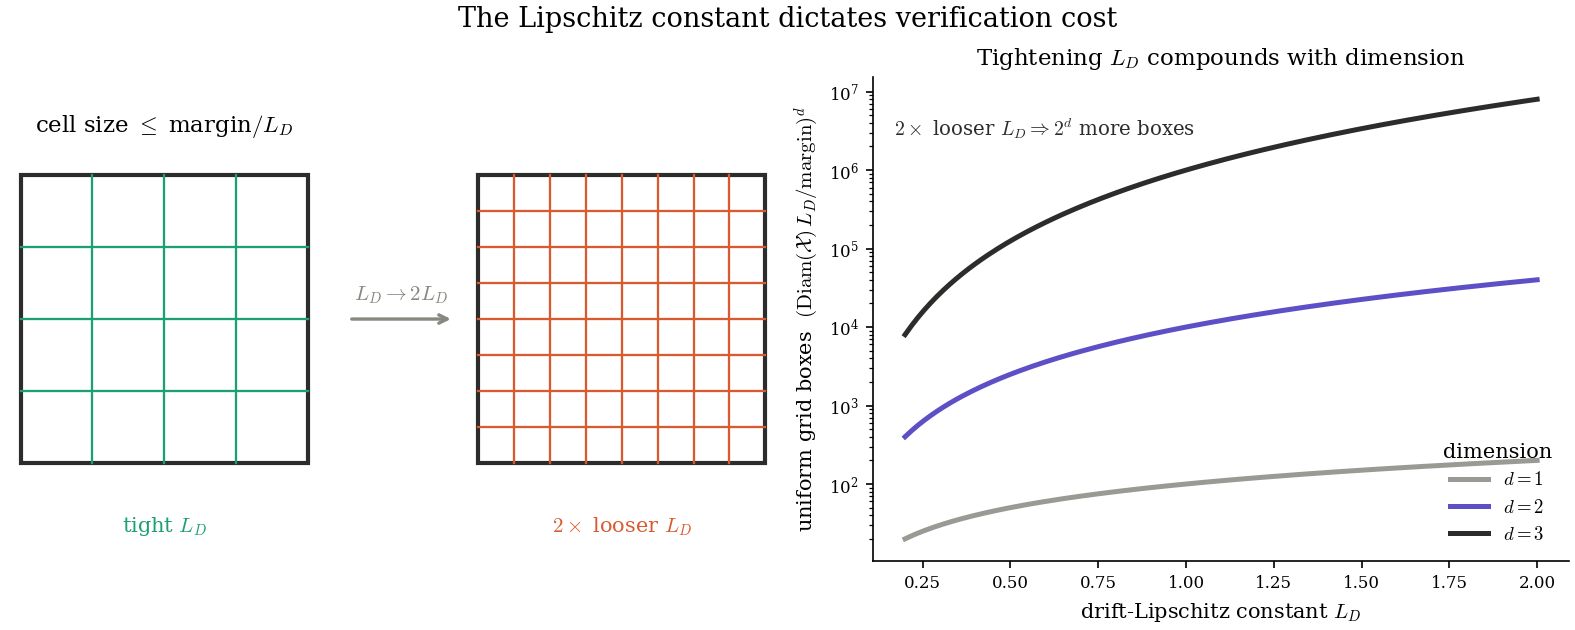
\includegraphics[width=0.92\linewidth]{Figures/lipschitz_gridding.png}
\caption{The Lipschitz constant dictates verification cost. \emph{Left:} each cell must be small
enough that the drift cannot cross the margin within it, so cell size $\lesssim\text{margin}/L$; a
looser constant forces a finer grid. \emph{Right:} the box count \eqref{eq:boxcount} grows as the
$d$-th power of $L$, so tightening the constant compounds with dimension.}
\label{fig:gridding}
\end{figure}

\subsection{The Margin Budget}
\label{subsec:budget}

Beyond forcing a finer grid, the Lipschitz constant caps the margin $\varepsilon$ one can certify at all. If $\cert$ is $L_\cert$-Lipschitz then $\expe_{x'}[|\cert(x)-\cert(x')|]\le L_\cert\,\expe_{x'}[\|x-x'\|]$, and a valid margin at $x$ obeys $\varepsilon(x) \le \cert(x)-\expe[\cert(x')]\le L_\cert\expe[\|x-x'\|]$; taking the binding (slowest-moving) state,
\begin{equation}
\label{eq:budget}
    \varepsilon \;\le\; L_\cert\,\inf_{x}\expe_{x'}[\|x-x'\|].
\end{equation}
This illustrates the maximally feasible decrease $\varepsilon$ that we can verify for the entire domain. The right-hand side is a property of the \emph{dynamics} (the smallest expected step), so the scale-free invariant is the ratio $\varepsilon/L_\cert$: a certificate cannot certify more decrease per unit of its own Lipschitz constant than the system actually moves. This highlights the dangers of using Lipschitz-constrained networks as certificates, as an $L_\cert$ that is too small will violate $\varepsilon / L_\cert \le \inf_{x}\expe_{x'}[\|x-x'\|]$, making the verification problem infeasible. Figure~\ref{fig:budget} illustrates this ``budget'' empirically; \cite{badings2025logRASM} attack the same tension from the certificate side, reparameterising it to lower its theoretical constant.

\begin{figure}[htbp]
\centering
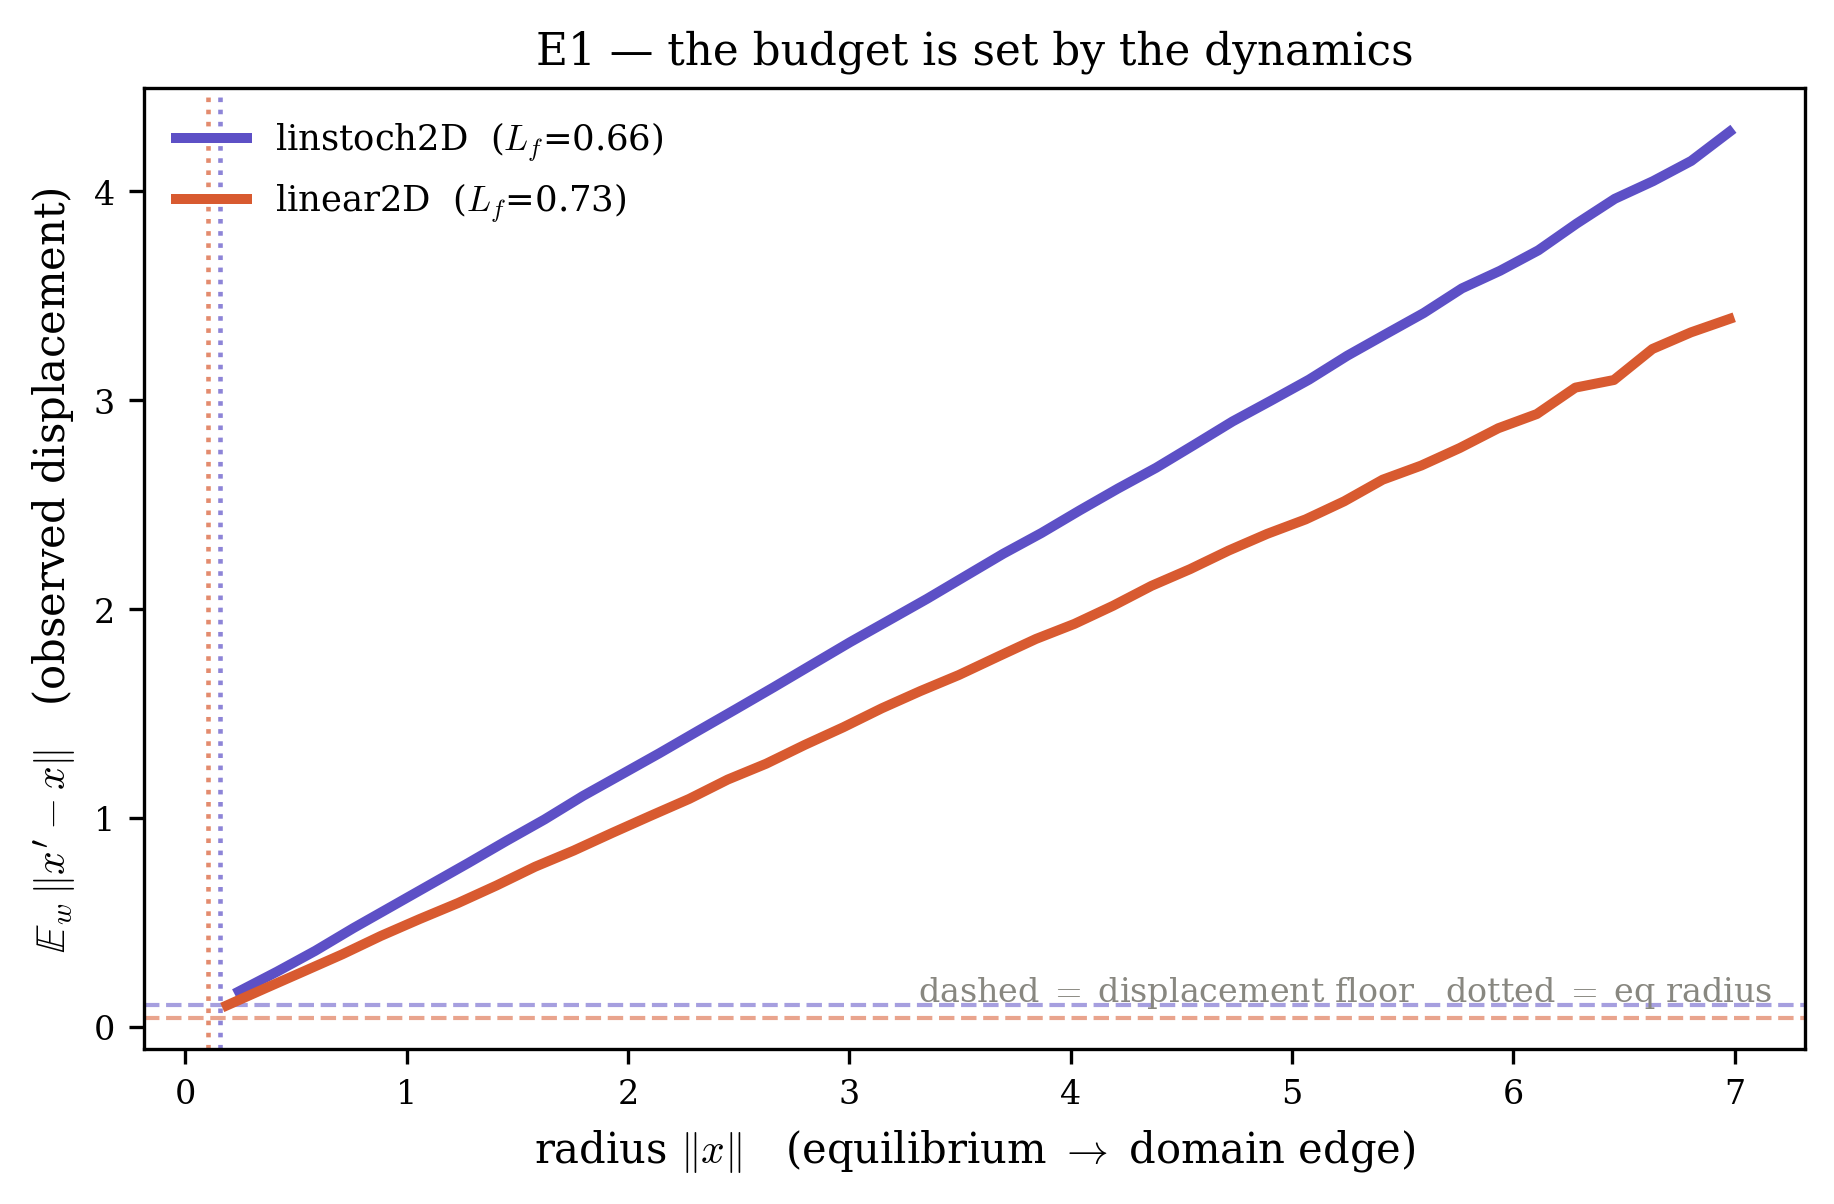
\includegraphics[width=0.64\linewidth]{Figures/lipschitz_budget_curve.png}
\caption{The budget \eqref{eq:budget} is set by the dynamics: the expected one-step displacement
$\expe_w\|x'-x\|$ rises from a floor near the equilibrium (which defines our domain-wide, fixed $\varepsilon$).}
\label{fig:budget}
\end{figure}


% ============================================================
\section{Tightening the Drift-Lipschitz Constant}
\label{sec:tightdrift}
% ============================================================

The sample-based verifiers in Section~\ref{sec:sampling-methods} consume one number: a sound upper bound on the drift-Lipschitz constant $L_\drift$. By \eqref{eq:boxcount} its magnitude drives an estimate on the cost to certify. To estimate $L_\drift$, one might derive a loose product bound $L_\drift \le L_\cert(L_f+1)$ via the composition bounds of \eqref{eq:lipschitz-composition} and Section~\ref{sec:nn_estimation}. However, we have established that composing global bounds is loose, assuming a worst-case alignment that inflates the discretisation error. We develop our tightenings in the deterministic setting of Section~\ref{subsec:gridding}, where the drift is $D$ \eqref{eq:det-drift} and the product bound reads $L_D \le L_\cert(L_f+1)$.

\subsection{Exact $L_D$ Computation}

For this contribution we assume that the dynamics $f$ are deterministic and linear, and $\cert$ is piecewise linear (for example a feed-forward $\mathrm{ReLU}$ network), with constant gradient $g_i$ on each activation region $R_i$. Given this, $\nabla D$ is piecewise constant.

\begin{proposition}[Exact drift-Lipschitz constant]
\label{prop:exactLD}
For linear $A$ and piecewise-linear $\cert$,
$\;L_D=\max\{\|A^\top g_j-g_i\| : R_i\cap A^{-1}R_j\cap\aX\neq\emptyset\}$.
\end{proposition}
\medskip\noindent\emph{Proof sketch.}\ $D$ is piecewise linear, so its Lipschitz constant is the maximum gradient norm over its linear pieces. Each piece is a nonempty cell $R_i\cap A^{-1}R_j\cap\aX$, on which $\nabla D=A^\top g_j-g_i$.\hfill$\square$\medskip

The exact constant improves on the product bound in two ways: it splits $\|A^\top g_j-g_i\|\le\|A\|\,L_\cert+L_\cert$ by the triangle inequality (the product bound discards the cancellation between the two terms), and it maximises over $i,j$ independently (the product bound discards that $x$ is the same point in both terms). Soundness of the estimate rests on a simple invariant: for any set $S$ containing every feasible pair, $\max_{(i,j)\in S}\|A^\top g_j-g_i\|\ge L_D$, so starting from all pairs and pruning only \emph{certifiably} infeasible ones can only tighten the bound, never break it. In practice we run LipBaB on the single network $D=\cert\circ A-\cert$; being anytime-sound, it returns a valid bound even on early termination.

\subsection{Results}

Table~\ref{tab:tightdrift} reports three sound upper bounds on $L_D$ for trained certificates on deterministic linear systems in $2$--$4$ dimensions ($\|A\|_\infty<1$, so the composition bounds are sound over the same box). M1 calculates $L_D$ by computing the product of spectral norms through the network (\eqref{eq:lipschitz-layer}) for $L_\cert$, which is then composed with $L_f$. M2 calculates $L_D$ in the same way, but uses LipBaB to compute the exact constant for $L_\cert$. Finally, M3 is the new proposition, where we use LipBaB to compute $L_D$ directly.

Running the branch-and-bound on the drift (M3) is consistently $1.3$--$1.5\times$ tighter than the best composition bound (M2) and $2.8$--$4.6\times$ tighter than the spectral product (M1). By \eqref{eq:boxcount} the M2$\to$M3 factor alone divides the box count by $(1.4)^d$, about $2\times$ in 2D and $3.8\times$ in 4D.

\begin{table}[htbp]
\centering
\begin{tabular}{cc rrr rr}
\hline
$d$ & $L_f$ & M1 spectral & M2 LipBaB & M3 drift & M1/M3 & M2/M3 \\
\hline
2 & 0.54 & 1.10 & 0.37 & 0.27 & $4.0\times$ & $1.4\times$ \\
2 & 0.60 & 1.60 & 0.52 & 0.38 & $4.3\times$ & $1.4\times$ \\
3 & 0.45 & 1.16 & 0.55 & 0.42 & $2.8\times$ & $1.3\times$ \\
4 & 0.55 & 1.78 & 0.92 & 0.60 & $2.9\times$ & $1.5\times$ \\
4 & 0.51 & 3.11 & 0.94 & 0.67 & $4.6\times$ & $1.4\times$ \\
\hline
\end{tabular}
\caption{Sound drift-Lipschitz estimates (upper bounds on $L_D$). M1 = product of spectral norms;
M2 = LipBaB on $\cert$ composed via $(L_f{+}1)$; M3 = LipBaB run on the drift $\cert\circ A-\cert$. M3 is uniformly
tightest.}
\label{tab:tightdrift}
\end{table}

\subsection{Anisotropic constants for free}
\label{subsec:aniso}


\paragraph{Directional constants.} Finally, a single global constant can be replaced by \emph{directional} ones. For a unit direction $v$, $L_f(v):=\sup_x\|J_f(x)\,v\|\le L$ is often far smaller, and for a scalar certificate it is one gradient projection to evaluate. We show that LipBaB yields these \emph{soundly}, and that they sharpen the verifier's discretisation.


LipBaB already computes, per leaf of its search, the exact per-region gradient; the per-axis constant $L_\cert(e_i)=\sup_x|\partial \cert/\partial x_i|$ is simply the component-wise maximum of those gradients over the (finitely many, fully enumerated) regions --- a \emph{sound} bound satisfying $L_\cert(e_i)\le L_\cert$. These anisotropic constants sharpen the discretisation: over an axis-aligned cell of side $w_i$ the sound bound $|\cert(x)-\cert(y)|\le\sum_i L_\cert(e_i)\,w_i$ replaces the isotropic $L_\cert\|w\|$, and refining each axis to its own sensitivity ($w_i\propto 1/L_\cert(e_i)$) reduces the box count from $\propto L_\cert^{\,d}$ to $\propto\prod_i L_\cert(e_i)$, a factor $\prod_i\big(L_\cert/L_\cert(e_i)\big)\ge 1$. We report the per-axis constants of the certificate; running LipBaB on the drift network $D=\cert\circ A-\cert$ (as in M3) yields the per-axis drift constants $L_D(e_i)$ by the identical extraction, and it is these that enter the box count \eqref{eq:boxcount}.

Table~\ref{tab:aniso} measures this on the same certificates. The per-axis constants are all below the global one and the reduction, being a product over axes, compounds with dimension: from $\approx1.5\times$ in 2D to $\approx8$--$17\times$ in 4D. Because it multiplies the M2$\to$M3 gain above, the two contributions stack.

\begin{table}[htbp]
\centering
\begin{tabular}{cc l r}
\hline
$d$ & $L_\cert$ (global) & per-axis $L_\cert(e_i)$ & box-count reduction \\
\hline
2 & 0.24 & $(0.22,\,0.18)$ & $1.5\times$ \\
2 & 0.32 & $(0.27,\,0.22)$ & $1.8\times$ \\
3 & 0.38 & $(0.36,\,0.20,\,0.18)$ & $4.1\times$ \\
4 & 0.60 & $(0.32,\,0.41,\,0.26,\,0.23)$ & $17.0\times$ \\
4 & 0.62 & $(0.41,\,0.46,\,0.40,\,0.26)$ & $7.8\times$ \\
\hline
\end{tabular}
\caption{Sound anisotropic (per-axis) Lipschitz constants extracted from LipBaB, and the resulting
axis-aligned box-count reduction $\prod_i(L_\cert/L_\cert(e_i))$. Every $L_\cert(e_i)\le L_\cert$; the saving
compounds with dimension.}
\label{tab:aniso}
\end{table}


% ============================================================
\section{Discussion}
% ============================================================

The two framings of this chapter are one picture. The Lipschitz constant is, to machine learning, a robustness quantity to estimate \cite{fazlyab2019lipsdp,bhowmick2021lipbab} and control \cite{miyato2018spectral,araujo2023unified}; to formal methods, the bridge that turns finite evidence into a whole-domain guarantee \cite{wu2020game,berkenkamp2017safe}. Certificate verification needs both at once, and because verification cost is a $d$-th power of the constant \eqref{eq:boxcount}, its magnitude is decisive. There are two levers: shrink the constant by controlling the architecture (Section~\ref{sec:control}), trading expressivity, or estimate it more tightly, changing nothing about the certificate but much about the cost of verifying it. Our two contributions take the second route on the exact object the verifiers consume --- the drift constant --- computing it directly rather than by composition, and extracting sound per-axis constants that sharpen the grid; because the two savings multiply, they reduce the box count by more than an order of magnitude in four dimensions. The core limitation is that both lean on the linearity that keeps the drift a $\mathrm{ReLU}$ network. Extending them to nonlinear dynamics, where the composed drift is no longer piecewise linear, is the clear next step, and would likely rely on another tool such as bound propagation.

\newpage
